\makeatletter
\@ifundefined{standalonetrue}{\newif\ifstandalone}{}
\@ifundefined{section}{\standalonetrue}{\standalonefalse}
\makeatother
\ifstandalone
\documentclass[11pt]{report}

/Users/evan/Karen/latex/all_usepackages.tex
\usepackage[margin=1.25in]{geometry}
\usepackage{xcolor}

% Sepia
%\definecolor{myBGcolor}{HTML}{F6F0D6}
%\definecolor{myTextcolor}{HTML}{4F452C}

\definecolor{myBGcolor}{HTML}{3E3535}
\definecolor{myTextcolor}{HTML}{CFECEC}
%\pagecolor{myBGcolor}
%\color{myTextcolor}

\begin{document}
\tableofcontents
\fi

{ \graphicspath{{rbffd_methods_content/}}

\chapter{Derivatives for RHS of Weight System}
We start with:
\begin{align} 
\psi (x,y) = e^{-\epsilon^2(x^2+y^2)} \cdot G_k(2\epsilon^2(x x_i +y y_i)) \label{eq:rbf_ga_basis}
\end{align}

Fornberg et al. \cite{FornbergLehtoPowell12} provide that derivatives of the basis functions requires:
\begin{align}
\pd{^p G_k(z)}{z^p} = G_{max(0,k-p)} (z), \ \ \ \ \ p = 0, 1, 2 \cdots 
\end{align}
and derivatives of Equation~\ref{eq:rbf_ga_basis} can be obtained via the \emph{product rule}. 

For RBF-GA, we have: 
\begin{align}
z & = 2\epsilon^2(x x_i + y y_i) \label{eq:gamma_z}
\end{align}

\section{$\pd{}{x}$}

First, we test derivation for $\pd{}{x}$. 

Apply the product rule: 
\begin{align}
\pd{\psi(x,y)}{x} & = \pd{}{x} \left( e^{-\epsilon^2(x^2+y^2)} \cdot G_k(z)  \right) \nonumber \\
& = \pd{}{x}\left( e^{-\epsilon^2 (x^2 + y^2)} \right) G_k(z) + e^{-\epsilon^2(x^2 + y^2)} \pd{G_k(z)}{x} \label{eq:x_product_rule}
\end{align}

Use the chain rule as necessary:
\begin{align}
\pd{}{x}\left( e^{-\epsilon^2 (x^2 + y^2)} \right) & = e^{-\epsilon^2 (x^2 + y^2)} \cdot \pd{}{x} \left( \epsilon^2(x^2+y^2) \right) \nonumber \\
        & = e^{-\epsilon^2 (x^2 + y^2)} \left(2x \epsilon^2 \right) \label{eq:x_part1}
\end{align}

%\begin{align}
%\pd{}{x} \left( \epsilon^2(x^2+y^2) \right) &= \pd{}{x}(\epsilon^2 x^2) + \pd{}{x}(\epsilon^2 y^2) \\
%&= 2x \epsilon^2 + 0
%\end{align}

\begin{align}
\pd{G_k(z)}{x} & = \pd{z}{x} \pd{}{z} G_k(z) \nonumber \\
               & = \pd{}{x} \left( 2\epsilon^2(x x_i + y y_i) \right) G_{max(0,k-p)}(z) \nonumber \\ 
               & = 2 \epsilon^2 x_i G_{max(0,k-p)}( z ) \label{eq:x_part2}
\end{align}
Note that in the derivative of $z$ we assume the center coordinates $x_i$ and $y_i$ are considered scalars. 


Finally, we substitute Equation~\ref{eq:x_part1} and \ref{eq:x_part2} into Equation~\ref{eq:x_product_rule} to get:
\begin{align}
\pd{\psi(x,y)}{x} & = \left( 2x\epsilon^2 G_k(z) + \pd{G_k(z)}{x} \right) e^{-\epsilon^2(x^2 + y^2)} \nonumber \\
                 & = \left( 2x\epsilon^2 G_k(z) + 2 \epsilon^2 x_i G_{max(0,k-p)}( z )  \right) e^{-\epsilon^2(x^2 + y^2)}  \nonumber \\
                 & = \left( x G_{k}(z) + x_i G_{max(0,k-p)}(z) \right) 2 \epsilon^2 e^{-\epsilon^2(x^2+y^2)}\label{eq:rbf_ga_xderiv}
\end{align}


\section{$\pd{}{y}$, and higher dimensions}

We repeat the process for $\pd{}{y}$, but due to similarity to $\pd{}{x}$, we can conclude: 

\begin{align}
\pd{\psi(x,y)}{y}   & = \left( y G_k(z) + y_i G_{max(0,k-p)}( z )  \right) 2\epsilon^2 e^{-\epsilon^2(x^2 + y^2)} \label{eq:rbf_ga_yderiv}
\end{align}
As the problem dimension increases, each first order derivative results similar equations, but a substitution for $r(\vx)^2 = (x^2 + y^2 + \cdots)$ can be made: 
\begin{align}
\pd{\psi(\vx)}{x}   & = \left( x G_k(z) + x_i G_{max(0,k-p)}( z )  \right) 2\epsilon^2 e^{-\epsilon^2 r(\vx)^2} \label{eq:rbf_ga_yderiv}
\end{align}


\section{Laplacian $\Laplacian$}

The Laplacian, $\Laplacian = \sum_{d=1}^{D}  \pdd{}{x_d}$ (where $D$ is the problem dimension) can be obtained following \cite{FornbergLehtoPowell12} to rewrite Equation~\ref{eq:rbf_ga_basis} as the product of two functions in one variable. 

\subsection{2D}

\subsection{3D}


\section{Projected Operators}

For the Stokes problem we need projected operators on the sphere. Derivation of these operators can be done via the chain rule, but I suspect that we may be able to compose the projected operators using only the basic operators for $\pd{}{x}$,  $\pd{}{y}$, and $\pd{}{z}$ as demonstrated in one of my dissertation Appendices---I was able to compose Differentiation Matrices for projected operators based on DMs for the unprojected operators with minimal loss of accuracy. 

In theory the composition/indirect approach to obtaining the projected operators will suffice. If not, we shall return to derive the RHS forms. 


}

%\part{Appendices}
%\appendix
%The following appendices are included to illuminate subtleties of the RBF-FD method. The first discusses the method's ability to avoid pole singularities when applied to solid body transport on the sphere. The second considers the difference between directly computing weights for differentiation operators versus leveraging linear combinations of weights to indirectly construct the same operators.
%\include{rbffd_avoid_pole_singularities}
%\include{rbffd_weights_on_sphere}

\section{Problems with Paper}
\begin{itemize}
%\item The size of matrix $B_k$---stated below Equation 14 in Bengt's paper---is wrong. The authors state that the dimensions are $\begin{pmatrix} d+k-1 \\ d-1 \end{pmatrix} \times \begin{pmatrix} d+k \\ d \end{pmatrix}$. While debugging I found that to reproduce the dimensions from Equations 12-14 requires the matrix $B_k$ to grow as (note: off by one on first dim): $\begin{pmatrix} d+k-1 \\ d \end{pmatrix} \times \begin{pmatrix} d+k \\ d \end{pmatrix}$


\item In Equations 12-14 in Bengt's paper, the growth rate for the power on the $\frac{1}{\epsilon^{*}}$ is not obvious. Through trial and error I was able to deduce that the power should scale as: $\frac{1}{\epsilon^{2k}}$ where $k$ is the same $k$ on $G_k$. 

My trial and error was naive, but I found that without the proper scaling, any changes to $\epsilon$ would impact the conditioning and magnitude of elements in the matrix. I did a simple solve of $A x = ones$ where $A$ was the LHS produced with RBF-GA. When $\epsilon$ would change, the values of $x$ would change scale as well. By fixing the power on the scaling to $2k$ I am able to input any value for $\epsilon$ (e.g. $1e-2 \rightarrow 1e-15$ and the values of $x$ change by a minuscule amount ($< 1e-9$).

\item When $z = 2\epsilon^2 x \cdot x_i$ is negative (i.e., the cases where stencil nodes are outside of first quadrant), the gammainc function in matlab returns NaN values. How do we handle the situation? 
\begin{itemize}
\item Actually, the problem is not when they are outside the first quadrant. Instead, it appears when the nodes span multiple quadrants (e.g., when in $[-1,1]^d$ instead of $[0,1]^d$).
\item Answer: The $imag(gammainc(z,k)) < 1e-15$ for all cases tested. . Since it is so near to 0, we simply exclude it by requesting the $real(gammainc(z,k))$ when producing the bases. 
\end{itemize}

\item I am attempting to generate figures similar to Figure 3. I am able to reproduce the basis functions for $\Psi_1(x), \Psi_2(x), \Psi_3(x)$, but the remainder do not reproduce the figures in the paper. 
\begin{itemize}
\item Note: I was playing with different node distributions (regular, hexagonal, halton), and I realized that the visualized bases depend on the stencil and node locations. Bengt's paper does not explicitly state what node distribution was used to produce that figure. But at least I am confident that the results in Figure~\ref{fig:psis_3d} (and the X-Y axes view in Figure~\ref{fig:psis_2d}) are correct for my node distributions.
\end{itemize}
\end{itemize}

\begin{figure}
\centering
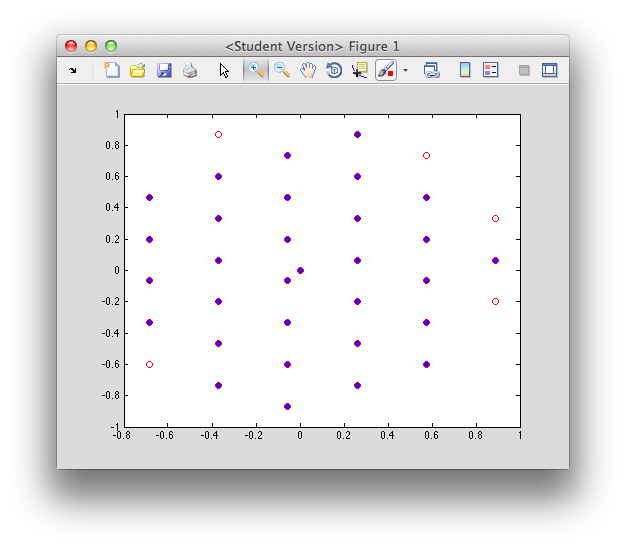
\includegraphics[width=0.55\textwidth]{./figures/hex_grid_stencil.png}
\caption{Red: A hexagonal grid within the unit disk ($r <= 1$). Blue: a stencil of size $n=31$ nodes selected from the grid. }
\label{fig:hex_grid_stencil}
\end{figure}

\begin{figure}
\centering
{\hskip-0.1\textwidth
\includegraphics[width=1.1\textwidth]{./figures/NewBasis_view3.eps}}
\caption{3D view of the new basis functions from RBF-GA for the hexagonal grid and stencil shown in Figure~\ref{fig:hex_grid_stencil} and stencil size $n=31$.}
\label{fig:psis_3d}
\end{figure}

\begin{figure}
\centering
{\hskip-0.1\textwidth
\includegraphics[width=1.1\textwidth]{./figures/NewBasis_view2.eps}}
\caption{2D view of the new basis functions from RBF-GA for the hexagonal grid and stencil shown in Figure~\ref{fig:hex_grid_stencil} and stencil size $n=31$.}
\label{fig:psis_2d}
\end{figure}


\ifstandalone
\bibliographystyle{plain}
\bibliography{merged_references}
\end{document}
\else
\expandafter\endinput
\fi
